\documentclass{standalone}
\usepackage{tikz}
\begin{document}
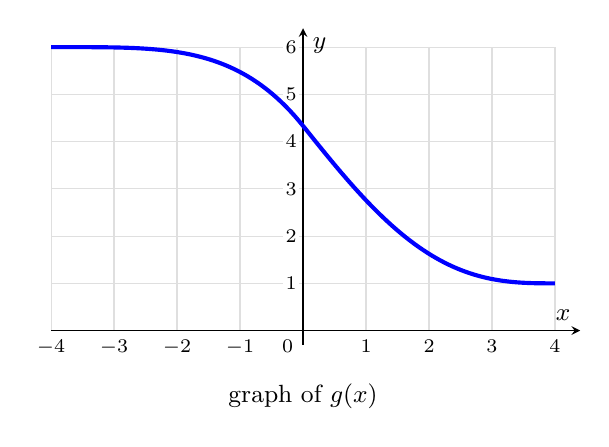
\begin{tikzpicture}[>=stealth, x=0.8cm, y=0.6cm,
    curve/.style={blue, line width=1.5pt}]
  % Graph of g on -4 <= x <= 4 (continuous, twice differentiable except at x = 0)
  % Curve pieces chosen to match the table values in the question:
  %   -4 <= x <= 0: g(x) = 6 - 5(x + 4)^4/768
  %    0 <= x <= 4: g(x) = 1 + (5/48)(4 - x)^3 - (5/384)(4 - x)^4
  %   g(-4) = 6, g(0) = 13/3, g(4) = 1, g'(-4) = g'(4) = 0, g'(0) = -5/3,
  %   g'' < 0 on (-4, 0), g'' > 0 on (0, 4), g''(-4) = g''(4) = 0
  \def\xmin{-4}\def\xmax{4}
  \def\ymin{-0.3}\def\ymax{6}

  % Light grid
  \draw[gray!25] (\xmin,0) grid[step=1] (\xmax,\ymax);

  % Axes
  \draw[->] (\xmin,0) -- (\xmax+0.4,0) node[above left, font=\small] {$x$};
  \draw[->] (0,\ymin) -- (0,\ymax+0.4) node[below right, font=\small] {$y$};
  \foreach \x in {-4,-3,-2,-1,1,2,3,4}
    \node[below, font=\scriptsize] at (\x,0) {$\x$};
  \node[below left, font=\scriptsize] at (0,0) {$0$};
  \foreach \y in {1,2,3,4,5,6}
    \node[left, font=\scriptsize, fill=white, inner sep=1pt] at (-0.05,\y) {$\y$};

  % Curve
  \draw[curve, samples=60, domain=-4:0]
    plot (\x, {6 - 5*(\x+4)^4/768});
  \draw[curve, samples=60, domain=0:4]
    plot (\x, {1 + (5/48)*(4-\x)^3 - (5/384)*(4-\x)^4});

  % Caption
  \node[font=\small] at (0,-1.4) {graph of $g(x)$};
\end{tikzpicture}
\end{document}
